\documentclass[12pt]{article}

%______________________PREAMBULO_________________________

%----------------------Paquetes--------------------------
\usepackage{amsmath,amssymb,amsfonts,latexsym,cancel}
\usepackage[spanish,es-tabla]{babel}
\usepackage[utf8]{inputenc}
%\usepackage[T1]{fontenc}
%\usepackage{lmodern}
\usepackage{mathpazo}             % Elige mathpazo O times, no ambos
% \usepackage{times}              % NO USAR ambos, mejor usa SOLO mathpazo o solo times (newtxtext,newtxmath)
\usepackage{csvsimple}
\usepackage{adjustbox}
\usepackage{graphicx}
\usepackage{geometry}
\usepackage{fancyhdr}
\usepackage{pstricks}
\usepackage{multicol}
\usepackage{tocbibind}
\usepackage{tabularx}\newcolumntype{Y}{>{\centering\arraybackslash}X}
\usepackage{listings}
\usepackage{xcolor}
\usepackage{siunitx}
\usepackage{verbatim}
%-------------Paquetes para el formato de las citas-------
\usepackage{float}
\usepackage{cite}
\usepackage{wrapfig}
\usepackage{apacite}
\usepackage[hyphens]{url}                   % ELIMINAR esta línea, limita usar solo hyperref
\usepackage[breaklinks,colorlinks=true,linkcolor=black,citecolor=blue, urlcolor=blue]{hyperref}

\lstset{ %
     language=C,                     % El lenguaje del código
     basicstyle=\ttfamily\footnotesize,  % Estilo básico del código
     keywordstyle=\color{blue},      % Color de las palabras clave
     commentstyle=\color{green},     % Color de los comentarios
     stringstyle=\color{red},        % Color de las cadenas
     numbers=left,                   % Colocar numeración de líneas a la izquierda
     numberstyle=\tiny\color{gray},  % Estilo de los números de línea
     stepnumber=1,                   % Numerar todas las líneas
     breaklines=true,                % Romper líneas largas automáticamente
     frame=single,                   % Colocar un marco alrededor del código
     captionpos=b,                   % Colocar el título del código abajo
}
\sisetup{
     round-mode = places,
     round-precision = 2 % Define el número de decimales que deseas
}
%-----------------------------ayuda de paquetes--------------------

\spanishdecimal{.}

%------------------------Margenes----------------------------

%\newgeometry{bottom = 2.5 cm, top = 2.5 cm, left = 2 cm, right = 2 cm} % Modifica el margen {Abajo, Arriba, Izquierda, Derecha

%----------------------------Interlineado----------------------------------

%\doublespacing
%\onehalfspace
%\singlespace
%\spacing{1.5} % Permite personalisar a gusto
%\setlength{\parskip}{2cm} % Es el espacio entre parrafos

%-----------------------------Sangria---------------------------------------

\setlength{\parindent}{0 cm} % Manipula la sangria
\setlength{\headheight}{14.5pt}

%---------------------Portada------------------

%\title{
%%\begin{figure}[h!]
%		
%%	\centering
%%	
\includegraphics[width=\linewidth]{Nom_UAdeC_FCFM.png}  			
%			
%%\end{figure}
%\huge \textbf{LABORATORIO DE FISICA 3}\\\LARGE TITULO PRACTICA\\}
%\author{ \Large \textbf{Profesor:}\\
%\Large \textbf{Alumno:} Oscar Joel Castro Contreras}
%\date{\today}

%--------------Encabezado y pie de pagina--------------------

\pagestyle{fancy}%Coloca el encabezado en el documento
\lhead[]{Física Moderna}%Encabezado izquierda
\rhead[]{Oscar Joel Castro Contreras}%Encabesado derecha
%\chead[]{}%Encabesado central
\renewcommand{\headrulewidth}{0.08 pt}%Coloca linea al pie de pagina

%\lfoot[]{PI}%Pie de pagina izquerdo
%\rfoot[]{PD}%Pie de pagina derecho
\cfoot[]{\thepage}%Pie de pagina central
\renewcommand{\footrulewidth}{0.08 pt}%Coloca linea al pie de pagina

%-----------------------------------------------------------------------------

\begin{document}
	
	\begin{titlepage}
	
		\centering
		{\bfseries
               {\scshape\LARGE El enlace molecular y enlace covalente \par}
		\par}
		%\vspace{1cm} 
		%{\LARGE Ensayo Tema 7\par}
		\vspace{1cm}
		{\LARGE \textbf{Oscar Joel Castro Contreras} \par}
          \vspace{0.5cm}
          {\large Cursos Propedéuticos Maestría En Ciencias Físicas\par}
          {\large Materia: Física Moderna\par}
		\vspace{1cm}
           
          %\vfill
          {\large (IFUAP Instituto de Física De La Universidad Autónoma De Puebla) \par}
		{\large (\Today) \par}
		\thispagestyle{empty}
		%\thispagestyle{fancy}
          \vspace{1cm}

	\end{titlepage}

     \newpage

     \thispagestyle{empty}

     \begingroup
     
     \renewcommand{\addtocontents}[2]{}
	
     \tableofcontents		

     \endgroup

     \newpage	

	\pagenumbering{arabic}
     \setcounter{page}{1} 	
	
     \section{Introducción}\label{sec:Introducción}
          \subsection{Enlace molecular}\label{sec:Enlace molecular}
               La interacción electrostática atractiva entre las cargas negativas de los electrones y las cargas positivas de los núcleos es responsable de mantienen los átomos juntos para formar moléculas, Las fuerzas magnéticas tienen solo un efecto débil en la cohesión y la fuerza gravitatoria son despreciables.\\\\
               Una molécula es un grupo de átomos eléctricamente neutros que se mantienen unidos con la fuerza suficiente como para tener como una sola partícula, una molécula de un tipo dado siempre tiene una cierta composición y estructura definidas.\\\\
               La moléculas de hidrógeno, siempre consisten en dos átomos de hidrógeno cada una, y las moléculas de agua siempre consisten en un átomo de oxígeno y dos átomos de hidrógeno cada una. Si uno de los átomos de una molécula se elimina de alguna manera o se une otro átomo, el resultado es una molécula de un tipo diferente con diferentes propiedades.\\\\
               Existe una molécula porque su energía es menor que la del sistema de átomos no interesantes separados. Si las interacciones entre un determinado grupo de átomos reducen su energía total, se puede formar una molécula. Si las interacciones aumentan su energía total, los átomos se repelan entre sí.\\\\
               Se han observado varios tipos de enlace que han sido descritos: Iónico, Metálico, Covalente, Sencillo, Múltiple, Polar, Apolar, Común, Dativo, de hidrógeno y otros. Se usaron diferentes propiedades físicas como la distancia, la energía y la dirección (ángulos de enlace), para decidir cuándo se presenta un enlace en una molécula.\\\\
               La distancia entre los núcleos de dos átomos enlazados es descrita por la distancia de enlace y frecuentemente este dato es tomado como criterio de que dos átomos están enlazados.\\\\
               Si la distancia entre los núcleos de dos átomos es menor que la suma de los radios de van der Waals de los dos átomos, se considera que hay un enlace entre ellos. Sin embargo, cuando la distancia interatómica es cercana a dicha suma existe una incertidumbre considerable, en particular porque el radio de van der Waals de un átomo es una cantidad definida pobremente, con una incertidumbre que es considerablemente mayor que la precisión con la cual es usualmente referida.\\\\
               A la energía necesaria para separar dos átomos en una molécula se le describe como energía de enlace y es también usada en ocasiones como criterio para decidir si existe un enlace entre ellos. Pero esta cantidad es difícil de determinar con exactitud.

          \subsection{Enlace metálico}\label{sec:Enlace metálico}
               Los metales sólidos poseen estructuras atómicas cristalinas bien definidas que en general están formados por un solo tipo de átomos. Estos conglomerados atómicos están unidos químicamente por un tipo de unión llamado enlace metálico. \\\\
               Las características físicas de los metales, como su elevada conductividad térmica y eléctrica, maleabilidad, ductilidad, brillo y tenacidad, los diferencian del resto de los elementos y compuestos. En una estructura metálica sólo pueden existir iones positivos (+) y una nube de electrones de valencia sin posición definida, que viajan por todo el conglomerado atómico.

               \begin{figure}[H]
                    \centering
                    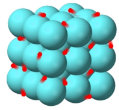
\includegraphics[height=2.5cm]{EnlaceMetalico.png}
                    \caption{Estructura de un metal.}
                    %\label{Fig:One-hot_endcoding_AF01}
               \end{figure}

               Esta disposición de los electrones les permite desplazase ante la aplicación de un potencial eléctrico, lo que explica la capacidad de los metales para conducir la corriente eléctrica.\\\\
               Entre las propiedades que podemos atribuirles a los metales, las más destacadas son las siguientes:
               
               \begin{itemize}
                    \item Tienen puntos de fusión y ebullición relativamente altos.
                    \item Se encuentran en estado sólido a temperatura ambiente.
                    \item Conducen el calor y la corriente eléctrica.
                    \item Son maleables y dúctiles.
                    \item Brillan peculiarmente.
                    \item Son bastante densos.
               \end{itemize}

               La maleabilidad es la capacidad de una sustancia para formar láminas, mientras que la ductilidad es la capacidad que tiene para formar hilos.\\\\
               \textbf{Aleaciones de metales}
               
               \begin{itemize}
               
                    \item El acero es la aleación de carbono con hierro, es posible que tenga algunas partes diminutas de ciertos compuestos metálicos como cromo o níquel y es muy fuerte, no se corroe.
                    \item El duraluminio es una aleación de cobre con aluminio y diferentes compuestos metálicos, esta tiene la propiedad de ser menos pesada pero de mayor dureza que el aluminio.
                    \item El latón es una aleación del zinc con el cobre y es de mucha utilidad para hacer planchas o tuberías.
               \end{itemize}
             
          \subsection{Enlaces iónico}\label{sec:Enlaces iónico}
               El enlace iónico es el tipo de unión que se forma cuando hay gran diferencia de electronegatividad entre los átomos mayor a 1.7, el elemento más electronegativo acepta los electrones del menos electronegativo para completar su octeto, pasando a formar un ion con carga negativa (anión), transformando al otro átomo en un catión, lo que da origen a su nombre. Este tipo de enlace también suele llamarse electrovalente, ya que es la fuerza electrostática la responsable del mantenimiento de su estructura.\\\\
               Si la cantidad de electrones que los dos átomos necesitaran perder o ganar para cumplir la regla del octeto no fuese la misma, deberían combinarse una relación de átomos de cada elemento que asegurara que la cantidades de electrones que un elemento necesita puedan ser aportados por el otro.\\\\
               Por ejemplo en la formación de NaF, donde cada átomo de azufre necesita dos electrones para llegar a tener 8 y cada átomo de sodio tiene solamente un electrón en su último nivel, por lo que se necesitarán dos átomos de sodio por cada átomo de azufre.

               \begin{figure}[H]
                    \centering
                    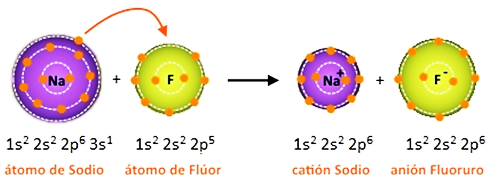
\includegraphics[height=5cm]{EnlaceIonico.png}
                    \caption{Esquema de la formación del enlace iónico.}
                    %\label{Fig:One-hot_endcoding_AF01}
               \end{figure}

               El enlace iónico es común entre metales de los grupos I y IIA con los no metales de los grupos VIA y VIIA, lo podemos representar con configuraciones electrónicas, modelos de Bohr o estructura de cargas.\\\\
               Los compuestos iónicos presentan diversas propiedades y características las cuales son:

               \begin{itemize}
                    \item Están formados por iones (+) y (-); metales y no metales.
                    \item Presentan punto de fusión y ebullición elevados.
                    \item Son sólidos a temperatura ambiente.
                    \item Forman cristales muy rígidos, donde los iones ocupan posiciones fijas.
                    \item Son solubles en agua.
                    \item No conducen la electricidad en estado sólido, pero si lo hacen cuando están disueltos en agua o cuando se los encuentra en estado fundido.
                    \item Son quebradizos.
               \end{itemize}

          \section{Desarrollo}\label{sec:Desarrollo}
               
               \subsection{Enlace covalente}\label{sec:Enlace covalente}
                    Este tipo de enlace se produce cuando la diferencia de electronegatividad entre los átomos que se combinan no es suficientemente grande. Si bien el elemento más electronegativo atraerá más los electrones del enlace no llegará a quitárselos al otro elemento, por lo que no se formarán iones y podríamos decir que los electrones que forman el enlace serán compartidos entre los dos átomos involucrados.\\\\
                    Son las fuerzas generadas entre átomos por compartición de pares de electrones, esto se debe a una deformación de los orbitales externos, la diferencia de electronegatividades $(\Delta EN)$ entre ellos es menor o igual a 1.7, son comunes entre no metales. Por la forma en que puede darse la covalencia los enlaces se clasifican en:

                    \begin{itemize}
                         \item No polares $\Delta EN = 0.4$
                         \item Polares $0.4 < \Delta EN < 1.7$
                         \item Coorinados $0.4 < \Delta EN < 1.7$
                    \end{itemize}

                    \subsubsection{Enlace covalente no polar}\label{sec:Enlace covalente no polar}
                         Este enlace ocurre entre átomos cuya diferencia de electronegatividad es igual a cero, en este caso la tendencia de los átomos para atraer electrones hacia su núcleo es igual, por lo tanto, el momento dipolar es cero. Por la cantidad de electrones de valencia de los átomos y su tendencia para completar 8 electrones estos pueden compartir 1, 2 o 3 pares de electrones generando los llamados enlaces simples, dobles y triples.

                    \subsubsection{Enlace covalente polar}\label{sec:Enlace covalente polar}
                         Se presenta cuando los átomos tienen $0.4 < \Delta EN < 1.7$ en este caso, el momento dipolar (“Momento dipolar: vector que actúa en la dirección del enlace molecular asimétrico. Las moléculas polares tienen momento dipolar permanente”) ya no es cero $(\mu \neq 0)$, pues el átomo más electronegativo atraerá el par de electrones enlazantes con más fuerza, esto significa que ese par girará durante más tiempo alrededor del núcleo más electronegativo, polarizando parcialmente la molécula.\\\\
                         La medición de los momentos dipolares proporciona evidencia experimental de la existencia de desplazamiento electrónico en los enlaces y distribución asimétrica de electrones en las moléculas. La magnitud del momento dipolar depende de la electronegatividad.
                    
                    \subsubsection{Enlace covalente coordinado}\label{sec:Enlace covalente coordinado}
                         Este enlace se presenta cuando solo uno de los átomos cede el par de electrones que comparten entre dos, el otro átomo sólo aporta su orbital vacío para acomodarlos.
                    
                    \subsubsection{Propiedades y características}\label{sec:Propiedades y características}
                         Las sustancias covalentes presentan las siguientes propiedades y características:

                         \begin{itemize}
                              \item Tienen gran variedad de puntos de fusión y ebullición.
                              \item Son aislantes térmicos y eléctricos.
                              \item Algunos son antiadherentes.
                              \item Sus moléculas tienen forma geométrica definida.
                              \item Existen en los tres estados de agregación: sólidos, líquidos y gaseosos.
                              \item Algunos tienen actividad química media y otros elevada.
                              \item Los polares son solubles en disolventes polares, los no polares son solubles en compuestos no polares.
                              \item No suelen conducir la electricidad.
                         \end{itemize}
     
     \nocite{*}
     \bibliographystyle{apacite}    
     \bibliography{Referencias_tema8}
     %\bibliography{Referencias_tema8}

\end{document}